\documentclass[10pt]{article}
\usepackage[a4paper,margin=18mm]{geometry}
\usepackage{graphicx,hyperref,amsmath,booktabs}
\hypersetup{colorlinks=true,urlcolor=blue}
\setlength{\parindent}{0pt}\setlength{\parskip}{6pt}
\begin{document}
\begin{center}\Large Curve25519 torus: guarded trace elimination\\[3pt]
\normalsize Native v1 --- 16 November 2026 --- unsigned producer evidence\end{center}
The Rust adapter reconstructs the original imaginary coordinate from a
real Chebyshev root and public label. All149776 fixed field-pair comparisons
agree with the original norm/power equations; all24 original toy members
also replay through the unchanged membership circuit.
Native PCC-20261116-35f196. [pcc:unverified]

\textbf{Exact chart and correspondence.}
Write $z=x+b\sqrt2$, $\omega=c+d\sqrt2$, $c^2-2d^2=1$ and $d\ne0$.
For an original norm-one $z$, the classical identities give
\[
T_q(x)^2-(x^2-1)U_{q-1}(x)^2=1,\qquad
z^q=T_q(x)+bU_{q-1}(x)\sqrt2.
\]
If $T_q(x)=c$, then $(x^2-1)U^2=2d^2$, and the unique original lift is
\[
b=\frac{(x^2-1)U}{2d},\qquad bU=d,\qquad x^2-2b^2=1.
\]
The implementation obtains $U=T'_q/q$ by binary automatic differentiation,
so it additionally excludes $q=0$ in the field. Native evaluated polynomial
identities support diagnosis; a formal proof of the adapter is not claimed.

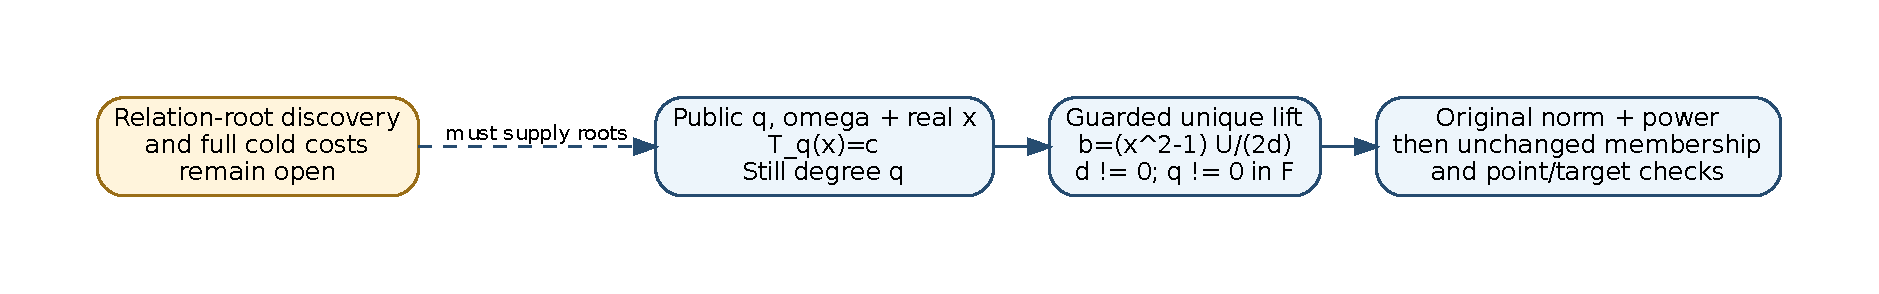
\includegraphics[width=\linewidth]{pipeline.pdf}

\textbf{Observed finite controls.} Each row checks every original pair $(x,b)$.
Original roots are counts over the stated labels, not timings or yield.
\begin{center}\begin{tabular}{lrrr}\toprule
Domain & Labels & Pair checks & Roots\\\midrule
$\mathbf F_{101}$, $q=3$, original &8&81608&24\\
$\mathbf F_{59}$, $q=3$, original &2&6962&6\\
$\mathbf F_{101}$, $q=1$, algebraic &2&20402&2\\
$\mathbf F_{101}$, $q=5$, algebraic &2&20402&2\\
$\mathbf F_{101}$, $q=17$, algebraic &2&20402&34\\\bottomrule
\end{tabular}\end{center}
The $q=5$ control distinguishes degree from rational root count. Splitting
requires the original exact-order and divisibility contracts.

\newpage
\begin{center}\Large Solver boundary and reproducible scope\end{center}
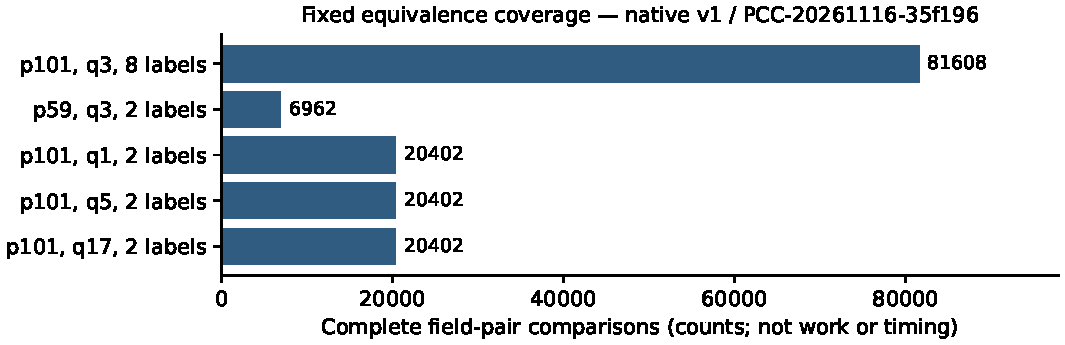
\includegraphics[width=\linewidth]{coverage.pdf}

\textbf{Actual-field and exceptional controls.}
Over $p=2^{255}-19$, eighteen chart cases comprise nine earlier $j/t$ parameters and their
nine conjugates. Conjugates use $\omega^{-1}$, outside the original positive
label set; these are separate algebraic controls. Every lift replays original
norm and power. Imaginary-coordinate mutations and six malformed/chart/
characteristic inputs reject. The excluded $\mathbf F_{101}$ case $q=3$,
$x=50$, $\omega=1$ has $T=1$, $U=0$: division by $d$ remains forbidden.
[pcc:unverified]

\textbf{Degree is retained.}
At the actual exponent $q=213156431$, the trace polynomial still has degree
$q$, while $U_{q-1}$ has degree $q-1$. Three narrow Lean endpoints apply the
existing Mathlib degree/derivative laws. Their hypotheses retain the
coefficient field and nonzero2 contracts; they do not prove the native AD,
coordinate lift, splitting or curve/group/compiler semantics.
Focused gate:3 named theorems,0 trusted-native; PCC-20261116-03a7ff.
[pcc:unverified]

The lift is a preconditioner interface, not a relation-root discovery
algorithm. Evaluating a compact recurrence does not price expansion into a
degree-$q$ polynomial or construction of its coordinate algebra. The next
solver must avoid the reference's triple enumeration, retain original roots
and charge setup, failed attempts, useful yield, indexing, selection,
kernel, scalar replay and memory to the one-target cold interval.

\textbf{Evidence and preservation.}
The49-source context reuses the unchanged43-input v2 archive and a new
six-input7452-byte delta. Six compiled-in hashes and the retained binary
qualifier match. The complete149776-byte comparison trace compresses to353
bytes with both digests retained. Release test/fmt/strict Clippy pass.
The first Rust API error and Lean call/cast/materialization failures remain
archived. All old source, criteria, reports, claims and direct Lean bindings
are unchanged. There was no timing, paid run, sampling or solver campaign.
[pcc:unverified]

\textbf{Sources and scope.}
\href{https://dlmf.nist.gov/18.5}{DLMF18.5.E1/E2} and
\href{https://dlmf.nist.gov/18.9}{18.9.T1}; pinned Mathlib Chebyshev source
\texttt{cfc55fc5}. Mathlib laws:\\
\texttt{natDegree\_T}, \texttt{natDegree\_U\_natCast} and
\texttt{T\_derivative\_eq\_U}. The historical native Chebyshev circuit
and unchanged consumer route criteria. KB runtime unavailable; direct sources
were read. No novelty is claimed for Chebyshev recognition or these laws.

See \texttt{trace-lift-v1/} protocol, derivation, source qualification,
native records and \texttt{lean-trace-v1/PROOF\_MAP.md}. Canonical scoreboard
and timeline are unchanged: no admitted performance datum was added.
\end{document}
